\documentclass{article}
\usepackage[utf8]{inputenc}
\usepackage{xcolor}
\usepackage{graphicx}
\usepackage{float}
\usepackage{minted}
\usepackage{circuitikz}
\usepackage{tikz}
\usetikzlibrary{shapes, arrows, calc, positioning, circuits.logic.US, circuits.logic.IEC}
\usepackage{geometry}
\geometry{a4paper, margin=1in}
\usepackage{hyperref}
\usemintedstyle{trac}

\usepackage{fancyhdr}
\pagestyle{fancy}
\fancyhf{}
\renewcommand{\headrulewidth}{0pt}
\fancyfoot[C]{\small 010153101 Digital Circuit and Microprocessor Fundamental \\ Semester 2/2025}
\fancyfoot[R]{\thepage}

% Redefine plain style to match fancy style (for the title page)
\fancypagestyle{plain}{%
  \fancyhf{}%
  \fancyfoot[C]{\small 010153101 Digital Circuit and Microprocessor Fundamental \\ Semester 2/2025}%
  \fancyfoot[R]{\thepage}%
  \renewcommand{\headrulewidth}{0pt}%
}

\title{Laboratory Exercise 6 - Week 1 \\ Latches and Flip-flops}
\author{}
\date{}

\begin{document}

\maketitle

The purpose of this exercise is to investigate latches, flip-flops, and registers.

\section*{Part I}

Intel FPGAs include flip-flops that are available for implementing a user's circuit. We will show how to make use of these flip-flops in Part IV of this exercise. But first we will show how storage elements can be created in an FPGA without using its dedicated flip-flops.

Figure 1 depicts a gated RS latch circuit. A style of VHDL code that uses logic expressions to describe this circuit is given in Figure 2. If this latch is implemented in an FPGA that has 4-input lookup tables (LUTs), then only one lookup table is needed, as shown in Figure 3a. The operation of the RS latch is behaviorally described in the characteristic table shown in Table \ref{tab:rs_latch_char}.

\begin{figure}[H]
    \centering
    % Placeholder for Figure 1: Gated RS Latch
    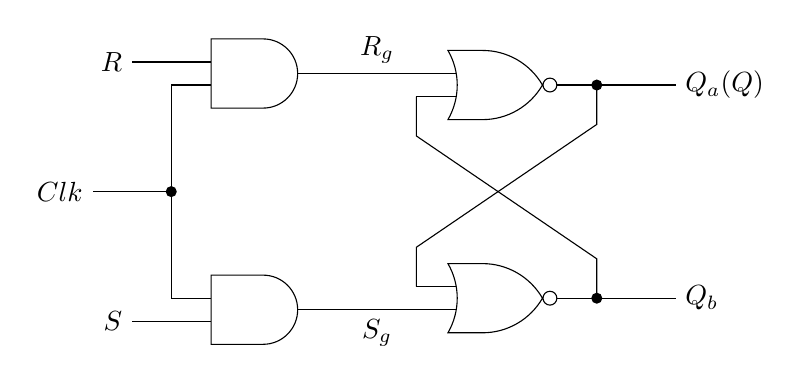
\begin{tikzpicture}[circuit logic US, huge circuit symbols]
    % Gates
    \node[and gate, inputs={nn}] (A1) at (0, 1.5) {};
    \node[and gate, inputs={nn}] (A2) at (0, -1.5) {};
    \node[nor gate, inputs={nn}, anchor=input 1] (O1) at ($(A1.output) + (2, 0)$) {};
    \node[nor gate, inputs={nn}, anchor=input 2] (O2) at ($(A2.output) + (2, 0)$) {};

    % Labels for internal signals (removed explicit nodes, added to paths below)

    % Inputs
    \draw (A1.input 1) -- ++(-1,0) node[left] {$R$};
    \draw (A2.input 2) -- ++(-1,0) node[left] {$S$};
    
    % Clock connection
    \draw (A1.input 2) -- ++(-0.5,0) coordinate (clk_top);
    \draw (A2.input 1) -- ++(-0.5,0) coordinate (clk_bot);
    \draw (clk_top) -- (clk_bot);
    \draw ($(clk_top)!0.5!(clk_bot)$) coordinate (clk_mid);
    \fill (clk_mid) circle (2pt);
    \draw (clk_mid) -- ++(-1,0) node[left] {$Clk$};

    % Connections to NOR latch with centered labels
    \draw (A1.output) -- node[above] {$R_g$} (O1.input 1);
    \draw (A2.output) -- node[below] {$S_g$} (O2.input 2);

    % Latch feedback with crossed lines
    \draw (O1.input 2) -- ++(-0.5, 0) coordinate (O1_fb_in);
    \draw (O2.input 1) -- ++(-0.5, 0) coordinate (O2_fb_in);

    % Feedback paths
    \draw (O1.output) -- ++(0.5,0) coordinate (Qa_out);
    \fill (Qa_out) circle (2pt);
    
    \draw (O2.output) -- ++(0.5,0) coordinate (Qb_out);
    \fill (Qb_out) circle (2pt);

    % Cross routing
    % Define intermediate points to avoid syntax errors
    \path (O2_fb_in) ++(-0,0.5) coordinate (O2_cross_x);
    \path (O1_fb_in) ++(-0,-0.5) coordinate (O1_cross_x);

    % Qa (Top) -> Bottom Input (O2)
    \draw (Qa_out) -- ++(0,-0.5) coordinate (Qa_drop) -- (O2_cross_x) -- (O2_fb_in);
    
    % Qb (Bottom) -> Top Input (O1)
    \draw (Qb_out) -- ++(0,0.5) coordinate (Qb_drop) -- (O1_cross_x) -- (O1_fb_in);

    % Outputs
    \draw (Qa_out) -- ++(1,0) node[right] {$Q_a (Q)$};
    \draw (Qb_out) -- ++(1,0) node[right] {$Q_b$};

\end{tikzpicture}

    \caption{A gated RS latch circuit.}
    \label{fig:gated_rs_latch}
\end{figure}

\begin{figure}[H]
    \centering
    \begin{minted}[frame=single, fontsize=\small, linenos]{vhdl}
LIBRARY ieee;
USE ieee.std_logic_1164.all;

ENTITY part1 IS
    PORT ( Clk, R, S : IN STD_LOGIC;
           Q : OUT STD_LOGIC);
END part1;

ARCHITECTURE Structural OF part1 IS
    SIGNAL R_g, S_g, Qa, Qb : STD_LOGIC ;
    ATTRIBUTE KEEP : BOOLEAN;
    ATTRIBUTE KEEP OF R_g, S_g, Qa, Qb : SIGNAL IS TRUE;
BEGIN
    R_g <= R AND Clk;
    S_g <= S AND Clk;
    Qa <= NOT (R_g OR Qb);
    Qb <= NOT (S_g OR Qa);
    Q <= Qa;
END Structural;
    \end{minted}
    \caption{Specifying the RS latch by using logic expressions.}
    \label{fig:vhdl_rs_latch}
\end{figure}

Although the latch can be correctly realized in one 4-input LUT, this implementation does not allow its internal signals, such as $R\_g$ and $S\_g$, to be observed, because they are not provided as outputs from the LUT. To preserve these internal signals in the implemented circuit, it is necessary to include a compiler directive in the code. In Figure 2 the directive KEEP is included by using a VHDL ATTRIBUTE statement to instruct the Quartus compiler to use separate logic elements for each of the signals $R\_g$, $S\_g$, $Qa$, and $Qb$. Compiling the code produces the circuit with four 4-LUTs depicted in Figure 3b.

\begin{figure}[H]
    \centering
    % Placeholder for Figure 3
    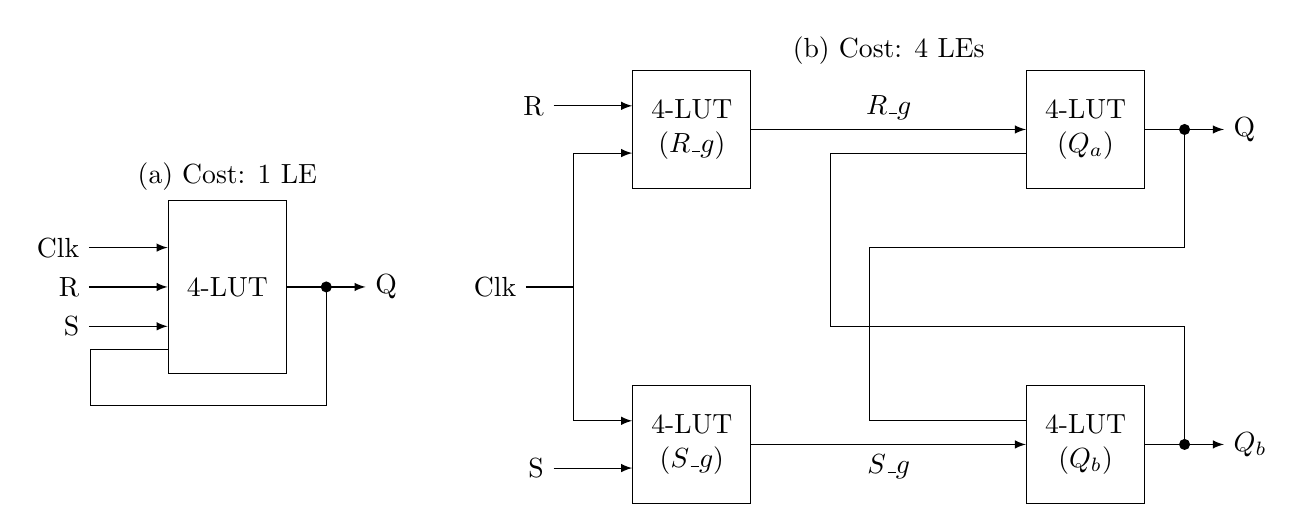
\begin{tikzpicture}[
    lut/.style={draw, rectangle, minimum width=1.5cm, minimum height=2.2cm, align=center},
    node distance=2cm,
    >=latex
]

% Part (a): Single 4-LUT
\node[lut] (lut1) at (0,0) {4-LUT};
\node[above] at (lut1.north) {(a) Cost: 1 LE};

% Inputs for (a)
\node (clk_a) [left=1cm of lut1.west, yshift=0.5cm] {Clk};
\node (r_a) [left=1cm of lut1.west] {R};
\node (s_a) [left=1cm of lut1.west, yshift=-0.5cm] {S};

\draw[->] (clk_a) -- (lut1.west |- clk_a.east);
\draw[->] (r_a) -- (lut1.west |- r_a.east);
\draw[->] (s_a) -- (lut1.west |- s_a.east);

% Outputs for (a)
\node (q_a) [right=1cm of lut1.east] {Q};
\draw[->] (lut1.east) -- (q_a);

% Feedback for (a)
\draw (lut1.east) ++(0.5,0) coordinate (qa_tap_a);
\fill (qa_tap_a) circle (2pt);
\draw (qa_tap_a) -- ++(0,-1.5) -- ++(-3,0) |- ([yshift=-0.8cm]lut1.west);
\node [left, font=\tiny] at ([yshift=-0.7cm]lut1.west) {};


% Part (b): Four 4-LUTs
% Positioning relative to (a)
\begin{scope}[xshift=5.9cm, yshift=2cm]
    \node at (2.5, 1) {(b) Cost: 4 LEs};

    % LUTs for R_g and S_g
    \node[lut, minimum height=1.5cm] (lut_rg) at (0, 0) {4-LUT \\ ($R\_g$)};
    \node[lut, minimum height=1.5cm] (lut_sg) at (0, -4) {4-LUT \\ ($S\_g$)};

    % Inputs for R_g and S_g
    % Inputs for R_g and S_g
    \node (r_b) [left=1cm of lut_rg.west, yshift=0.3cm] {R};
    \node (s_b) [left=1cm of lut_sg.west, yshift=-0.3cm] {S};
    
    % Common Clock
    \node (clk_common) at (-2.5, -2) {Clk};

    \draw[->] (r_b) -- (lut_rg.west |- r_b.east);
    \draw[->] (s_b) -- (lut_sg.west |- s_b.east);

    % Clock connections
    \draw (clk_common) -- (-1.5, -2);
    \draw[->] (-1.5, -2) |- ([yshift=-0.3cm]lut_rg.west);
    \draw[->] (-1.5, -2) |- ([yshift=0.3cm]lut_sg.west);

    % LUTs for Qa and Qb
    \node[lut, minimum height=1.5cm] (lut_qa) at (5, 0) {4-LUT \\ ($Q_a$)};
    \node[lut, minimum height=1.5cm] (lut_qb) at (5, -4) {4-LUT \\ ($Q_b$)};

    % Wiring R_g to Qa and S_g to Qb
    \draw[->] (lut_rg.east) -- node[above] {$R\_g$} (lut_qa.west);
    \draw[->] (lut_sg.east) -- node[below] {$S\_g$} (lut_qb.west);

    % Cross-coupling
    % Output Qa feeds back to Qb
    % Output Qb feeds back to Qa
    
    % Outputs
    \node (qa_out) [right=1cm of lut_qa.east] {Q};
    \draw[->] (lut_qa.east) -- (qa_out);
    \node (qb_out) [right=1cm of lut_qb.east] {$Q_b$};
    \draw[->] (lut_qb.east) -- (qb_out);

    % Feedback connections
    % From Qa output to Qb input
    \draw (lut_qa.east) ++(0.5,0) coordinate (qa_tap);
    \fill (qa_tap) circle (2pt);
    \draw (qa_tap) -- ++(0,-1.5) -- ++(-4,0) |- ([yshift=0.3cm]lut_qb.west);

    % From Qb output to Qa input
    \draw (lut_qb.east) ++(0.5,0) coordinate (qb_tap);
    \fill (qb_tap) circle (2pt);
    \draw (qb_tap) -- ++(0,1.5) -- ++(-4.5,0) |- ([yshift=-0.3cm]lut_qa.west);

\end{scope}

\end{tikzpicture}

    \caption{Implementation of the RS latch from Figure 1.}
    \label{fig:rs_latch_impl}
\end{figure}


\begin{table}[H]
    \centering
    \begin{tabular}{|c|c|c|c|c|}
        \hline
        Clk & R & S & Q(t+1) & Description \\
        \hline
        0 & x & x & Q(t) & Hold \\
        1 & 0 & 0 & Q(t) & Hold \\
        1 & 0 & 1 & 1 & Set \\
        1 & 1 & 0 & 0 & Reset \\
        1 & 1 & 1 & x & Indeterminate \\
        \hline
    \end{tabular}
    \caption{Characteristic table of the Gated RS Latch.}
    \label{tab:rs_latch_char}
\end{table}

Create a Quartus project for the RS latch circuit as follows:
\begin{enumerate}
    \item Create a new Quartus project for your DE0-CV board.
    \item \textbf{First, implement the circuit using Schematic Design.} Draw the circuit using the Block Editor and appropriate logic gates.
    \item Compile the schematic design and perform a functional simulation to verify its correctness. Ensure the behavior matches the expected RS latch operation.
    \item \textbf{Next, implement the circuit using Structural VHDL Design.}
    \item Generate a VHDL file with the code in Figure 2 and include it in the project.
    \item Compile the code. Use the Quartus RTL Viewer tool to examine the gate-level circuit produced from the code, and use the Technology Map Viewer tool to verify that the latch is implemented as shown in Figure 3b.
    \item Simulate the behavior of your VHDL code by using the simulation feature provided in the Quartus software. First, create a vector waveform file (*.vwf) using the Quartus software to specify the inputs and outputs of your circuit. Then, use the commands available in the Quartus Simulation Waveform Editor tool to run a simulation of the circuit. The resulting waveforms should look similar to those shown in Figure \ref{fig:sim_rs_latch}.
\end{enumerate}

\begin{figure}[H]
    \centering
    % Placeholder for Figure 4
    \input{tex/lab6p1_rs_latch_timing.tex}
    \caption{Expected waveforms for the RS latch.}
    \label{fig:sim_rs_latch}
\end{figure}

\section*{Part II}

Figure 5 shows the circuit for a gated D latch. Its corresponding characteristic table is provided in Table \ref{tab:d_latch_char}.

\begin{figure}[H]
    \centering
    % Placeholder for Figure 5: Gated D Latch
    \input{tex/lab6p2_gated_d_latch.tex}
    \caption{Circuit for a gated D latch.}
    \label{fig:gated_d_latch}
\end{figure}


\begin{table}[H]
    \centering
    \begin{tabular}{|c|c|c|c|}
        \hline
        Clk & D & Q(t+1) & Description \\
        \hline
        0 & x & Q(t) & Hold \\
        1 & 0 & 0 & Reset \\
        1 & 1 & 1 & Set \\
        \hline
    \end{tabular}
    \caption{Characteristic table of the Gated D Latch.}
    \label{tab:d_latch_char}
\end{table}

Perform the following steps:
\begin{enumerate}
    \item Create a new Quartus project.
    \item \textbf{First, implement the circuit using Schematic Design.} Draw the circuit using the Block Editor.
    \item Compile the schematic design and perform a functional simulation to verify its correctness.
    \item \textbf{Next, implement the circuit using Structural VHDL Design.}
    \item Modify the VHDL code from Part I to implement the gated D latch. Use the KEEP directive to ensure that separate logic elements are used to implement the signals R, S\_g, R\_g, Qa, and Qb.
    \item Compile your project and then use the Technology Map Viewer tool to examine the implemented circuit.
    \item Verify that the latch works properly for all input conditions by using functional simulation. Examine the timing characteristics of the circuit by using timing simulation.
    \item Create a new Quartus project which will be used for implementation of the gated D latch on your DE0-CV board. This project should consist of a top-level module that contains the appropriate input and output ports (pins) for your board. Instantiate your latch in this top-level module. Use switch SW0 to drive the D input of the latch, and use SW1 as the Clk input. Connect the Q output to LEDR0.
    \item Include the required pin assignments and then compile your project and download the compiled circuit onto your DE0-CV board.
    \item Test the functionality of your circuit by toggling the D and Clk switches and observing the Q output.
\end{enumerate}

\section*{Part III}

Figure 6 shows the circuit for a master-slave D flip-flop. The characteristic table for this negative-edge triggered flip-flop is shown in Table \ref{tab:ms_ff_char}.

\begin{figure}[H]
    \centering
    % Placeholder for Figure 6: Master-Slave D Flip-Flop
    \begin{circuitikz}
    \ctikzset{logic ports=ieee}
    \ctikzset{flipflops/scale=1}
    % Define standard D Latch style
    \tikzset{d-latch/.style={flipflop, flipflop def={
        t1=D, t3=C, t4={\ctikztextnot{Q}}, t6=Q
    }}}
    % Define Negated Enable D Latch style (for Slave)
    \tikzset{d-latch-n/.style={flipflop, flipflop def={
        t1=D, t3=C, t4={\ctikztextnot{Q}}, t6=Q
    }}}

    % Master Latch (Active High Enable)
    \node[d-latch] (Master) at (0,0) {Master};
    
    % Slave Latch (Active Low Enable via Bubble)
    \node[d-latch-n] (Slave) at (5,0) {Slave};
    
    % Inputs
    % Input D
    \draw (Master.pin 1) -- ++(-1.5, 0) coordinate (D_in) node[left] {D};
    
    % Clock Input common point
    % Align Clock horizontal start point with D node x-coordinate
    \coordinate (Clk_pin) at (Master.pin 3);
    
    % Clock Source
    \coordinate (Clk_in_Node) at ($(D_in) + (0,-2.5)$); % Lower down
    \draw (Clk_in_Node) node[left] {Clk} -- ++(1.5,0) coordinate (clk_main_split);
    \fill (clk_main_split) circle (2pt);
    
    % Connect Clock to Master Enable (Active High)
    % Route: Split -> Right -> Up -> Master Pin 3
    \draw (clk_main_split) -| (Master.pin 3);
    
    % Connect Clock to Slave Enable (Active Low)
    % Route: Split -> Right -> Right -> Up -> Slave Pin 3
    \draw (clk_main_split) -- ++(3,0) node[not port,anchor=in,scale=0.5] (not_port) {};
    \draw (not_port.out) -| (Slave.pin 3);
    
    % Logic:
    % Clk=1: Master En (Transp), Slave Dis (Hold).
    % Clk=0: Master Dis (Hold), Slave En (Transp).
    % Negative Edge Triggered.

    % Wiring Master Q -> Slave D
    \draw (Master.pin 6) -- (Slave.pin 1);
    
    % Outputs
    \draw (Slave.pin 6) -- ++(1, 0) node[right] {$Q$};
    \draw (Slave.pin 4) -- ++(1, 0) node[right] {$\bar{Q}$};

\end{circuitikz}

    \caption{Circuit for a master-slave D flip-flop.}
    \label{fig:master_slave_ff}
\end{figure}


\begin{table}[H]
    \centering
    \begin{tabular}{|c|c|c|c|}
        \hline
        Clk & D & Q(t+1) & Description \\
        \hline
        $\downarrow$ & 0 & 0 & Reset \\
        $\downarrow$ & 1 & 1 & Set \\
        0 & x & Q(t) & Hold \\
        1 & x & Q(t) & Hold \\
        \hline
    \end{tabular}
    \caption{Characteristic table of the Master-Slave D Flip-Flop (Negative-Edge Triggered).}
    \label{tab:ms_ff_char}
\end{table}

Perform the following:
\begin{enumerate}
    \item Create a new Quartus project.
    \item \textbf{First, implement the circuit using Schematic Design.} Create a symbol for the Gated D latch from Part II and use it to build the circuit.
    \item Compile the schematic design and perform a functional simulation to verify its correctness.
    \item \textbf{Next, implement the circuit using Structural VHDL Design.}
    \item Create a VHDL entity/component for the gated D latch from Part II. Then, write a top-level VHDL file that instantiates two copies of this component to implement the master-slave flip-flop.
    \item Include in your project the appropriate input and output ports for your DE0-CV board. Use switch SW0 to drive the D input of the flip-flop, and use SW1 as the Clock input. Connect the Q output to LEDR0.
    \item Include the required pin assignments and then compile your project.
    \item Use the Technology Viewer to examine the D flip-flop circuit, and use simulation to verify its correct operation.
    \item Download the circuit onto your DE0-CV board and test its functionality by toggling the D and Clock switches and observing the Q output.
\end{enumerate}

\vspace{1cm}
\noindent \textbf{Updated By:} R. Sutthaweekul \\
\textbf{Release Date:} 2026-01-01

\end{document}
